\documentclass[onecolumn]{IEEEtran}

% Basic required LaTeX packages
\usepackage[english]{babel} 
\usepackage[utf8]{inputenc} 
\usepackage[T1]{fontenc}

% Packages which allow format customisation
\usepackage{titling}
\usepackage{cite}
\usepackage{caption}
\usepackage{textcomp}
\usepackage{xcolor}
\usepackage{etoolbox} 
\patchcmd{\section}{\centering}{}{}{} % uses the etoolbox package to left align section headings

% Packages which help display things like maths and images correctly
\usepackage{amsmath,amssymb,amsfonts}
\usepackage{algorithmic}
\usepackage{graphicx}
\usepackage{hyperref}

\usepackage{subcaption}

% All your code should be in between the \begin{document} and \end{document} tags otherwise your compiler willl throw an error
\begin{document}


\title{Smart Home Adapters - Project Plan}
\author{Ben Sheffield, Theo Olausson, Gwion Ap Rheinallt, Luke Drennan, \\Guanghui Han, Sameer Karim, David Wang, Spencer Mccann}
\date{25/01/2019} % Leave blank to omit date. Comment out to include today's date or you can add a specific date

\maketitle

\section{Concept}
Smart home adapters transform the user’s existing tech into smart devices. The adapters will come with a selection of grips which can be swapped out to perform the different actions. Users will select the type of devices our product will be interacting with, such as a dial, switch, or button, and then our adapter will switch, twist or press to perform the desired operation. Going further we plan to integrate our device with other smart home solutions such as Alexa and IFTTT (If this then that) to provide a cohesive smart home experience.

For this project we are focusing on 3 use cases:

\begin{itemize}
    \item \textbf{Smart thermostat:} Current devices such as the Hive and Nest replace your existing thermostat, thus requiring landlord’s permission. Our device would go over your existing thermostat, reaching an audience not served by the competition.
    \item \textbf{Switches:} Existing products such as Philips Hue bulbs allow you to turn on/off and change the colour of your lights however they only support the most common bulb types. Our product goes over the existing light switch and is therefore compatible with all bulb types. This is not just useful for lights, but any switch. Often there are switches hidden behind appliances in hard to reach places, for example, a fridge in the garage. Our adapters connect with the user’s devices wirelessly, alleviating the need to pull out the fridge just to turn it off when not in use.
    \item \textbf{Bolt locks:} A linear sliding grip would allow a user to control a garden gate or other bolt lock mechanism. This could be useful for unlocking the gate for the delivery driver when you’re away from home. Again, existing solutions are not applicable to people living in rented homes.
\end{itemize}

\begin{figure}
    \centering
    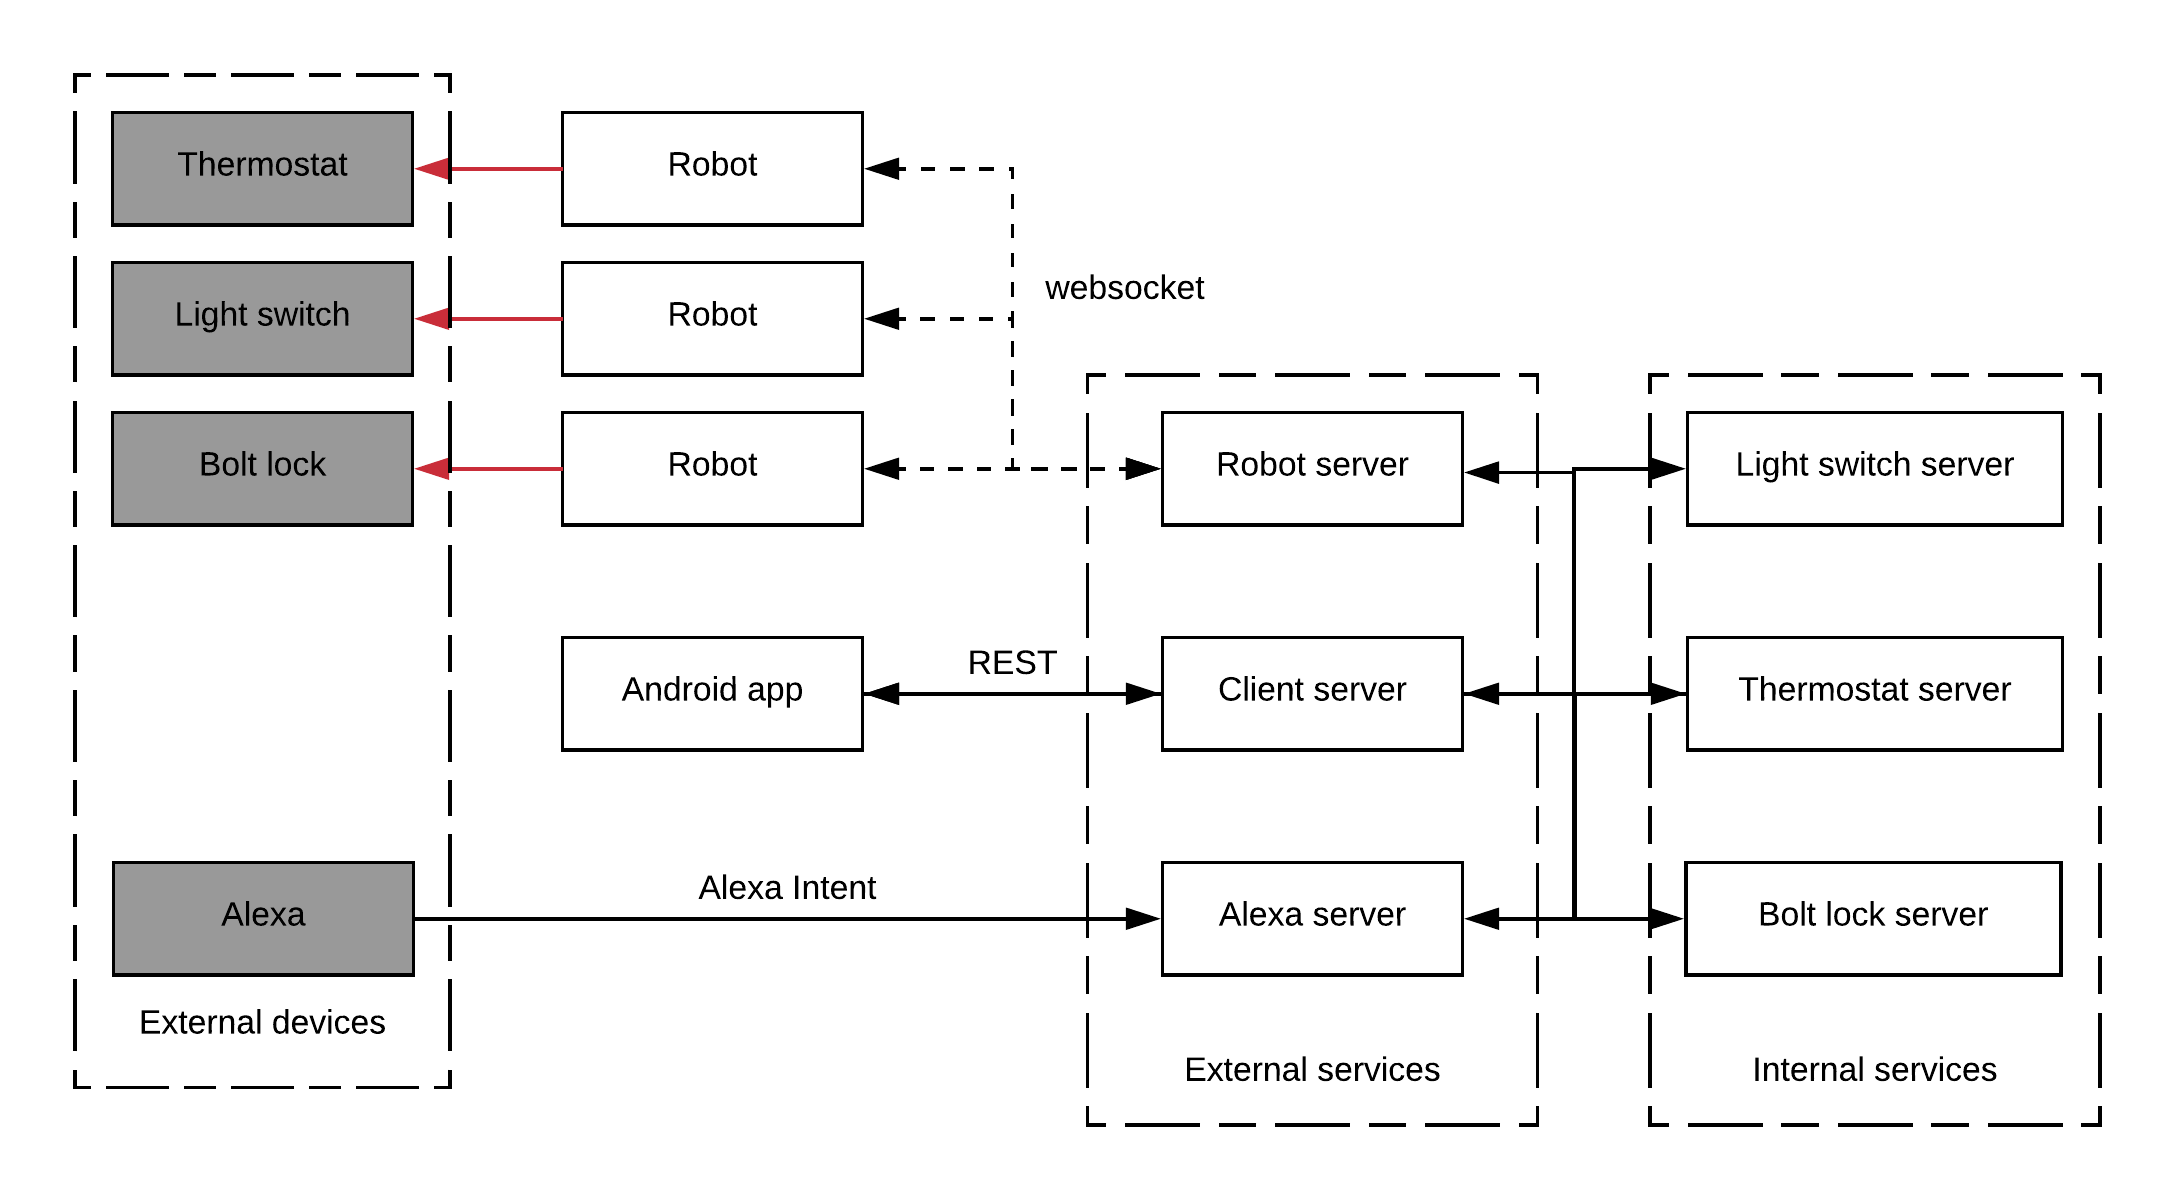
\includegraphics[width=1.0\linewidth]{architecture.png}
    \caption{Architecture of our system.}
\end{figure}

\subsection{Robot}

The robot is split into 2 parts: the controller and the grips. The controller includes an Arduino, an array of sensors, servo and a battery pack. The grips attach to the controller, when the servo turns the grips manipulate whatever device they are interacting with. The robots themselves attach to the devices with self-adhesive, thus they can easily be removed.

\begin{figure}
    \begin{subfigure}{.5\textwidth}
      \centering
      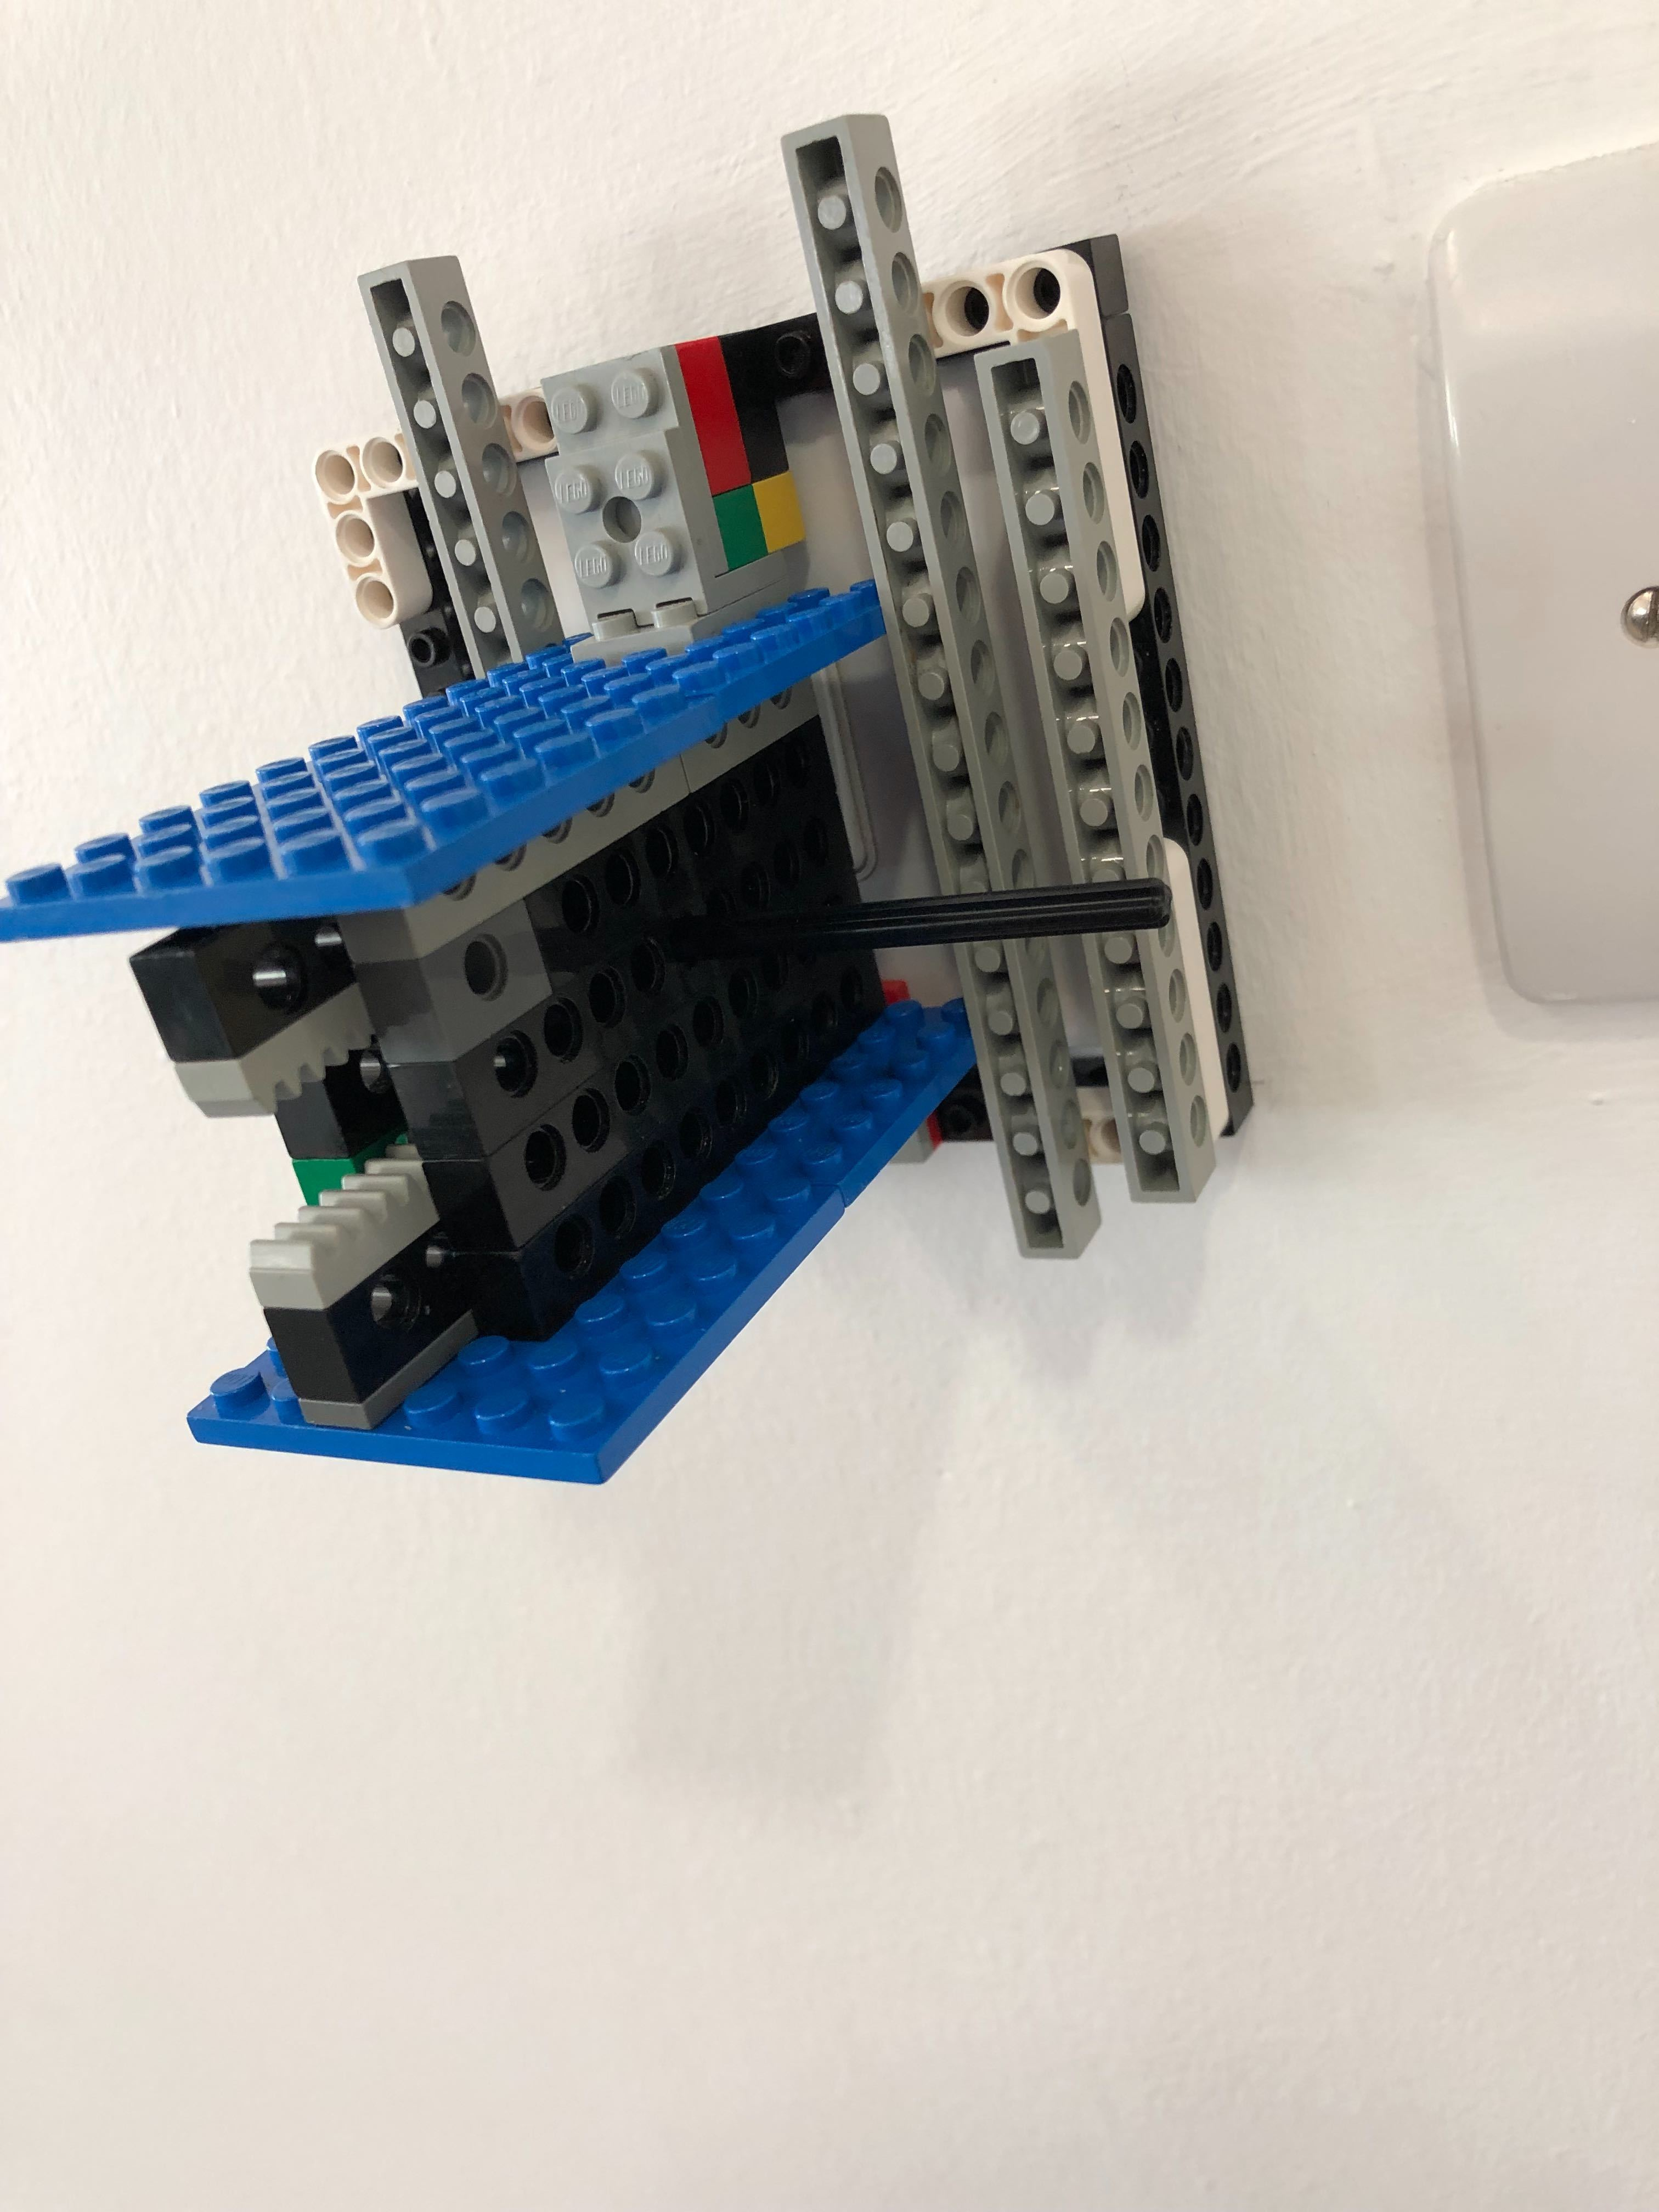
\includegraphics[width=.8\linewidth]{light-grip-1.jpg}
    \end{subfigure}
    \begin{subfigure}{.5\textwidth}
      \centering
      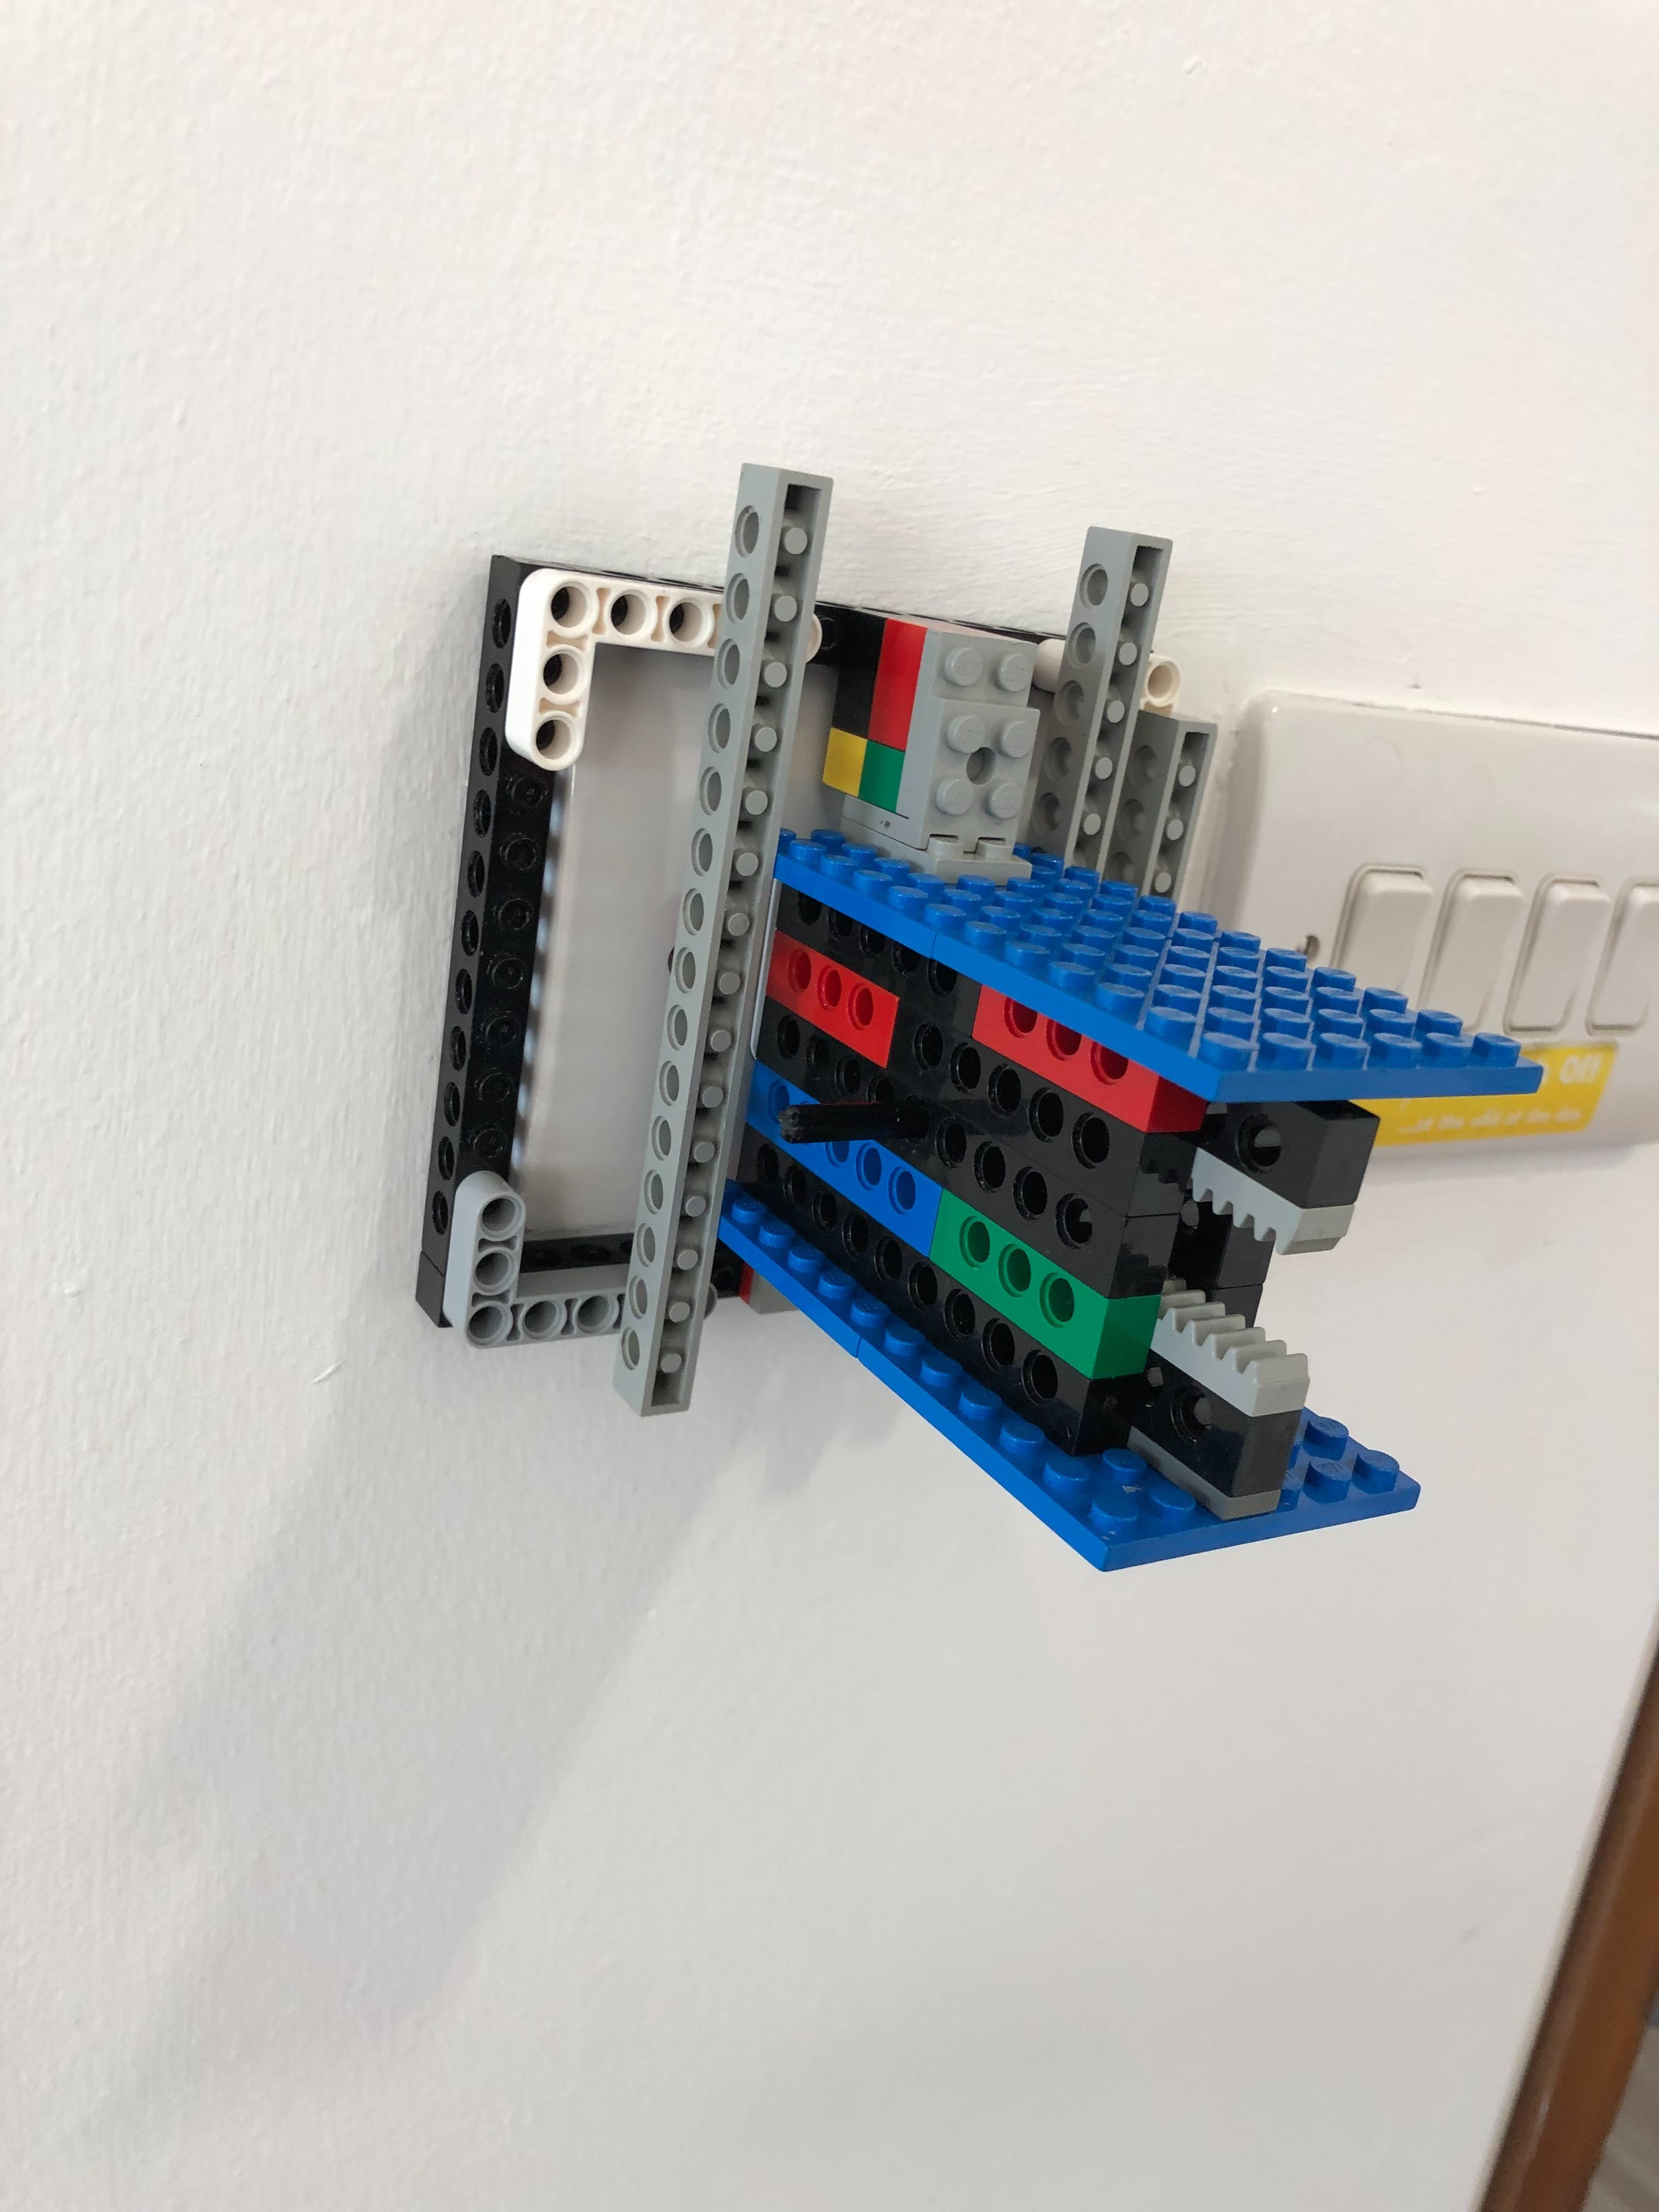
\includegraphics[width=.8\linewidth]{light-grip-2.jpg}
    \end{subfigure}
    \caption{First iteration of a light switch grip.}
    \label{fig:fig}
\end{figure}

\subsection{Web server}

The web server is actually a collection of many smaller web servers since we will be following the microservice architecture. The publicly accessible servers are:

\begin{itemize}
    \item The android app receives data and sends commands via our client API served via the client server. 
    \item Alexa sends alexa requests to our alexa server.
    \item The robot is connected via a web socket to the root server
\end{itemize}

The internal services correspond to each of the use cases. They keep track of the state the device is in, what actions can be performed, and what servo commands need to be sent. This architecture would allow us to point to user made use cases in the future.

\subsection{Android app}

The android app is the primary user interface into our system. It allows the user to register, calibrate and control their robots.

\begin{figure}
    \begin{subfigure}{.33\textwidth}
      \centering
      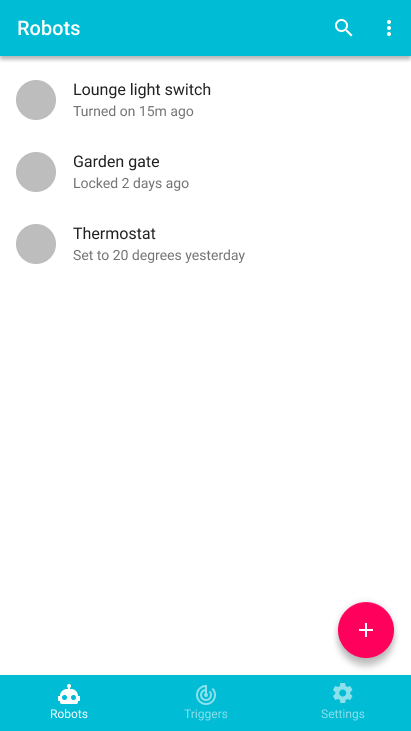
\includegraphics[width=.9\linewidth]{app-1.png}
    \end{subfigure}
    \begin{subfigure}{.33\textwidth}
        \centering
        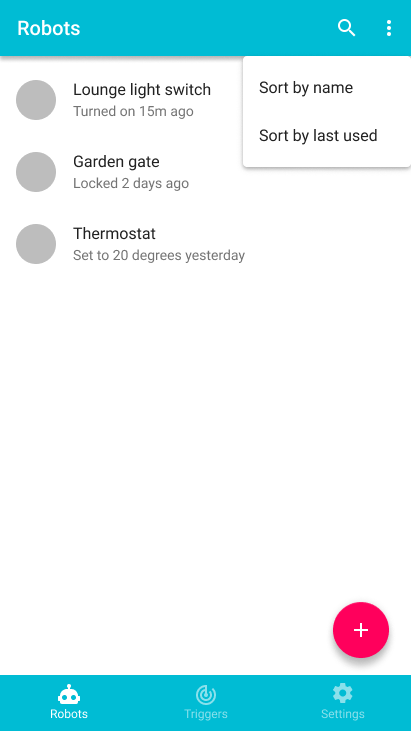
\includegraphics[width=.9\linewidth]{app-2.png}
    \end{subfigure}
    \begin{subfigure}{.33\textwidth}
        \centering
        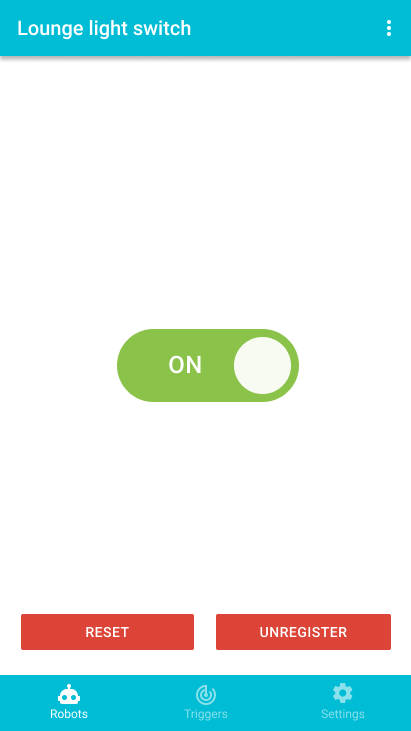
\includegraphics[width=.9\linewidth]{app-3.png}
    \end{subfigure}
    \caption{Quick mockup of the Android app.}
    \label{fig:fig}
\end{figure}

\end{document}